%% ----------------------------------------------------------------
%% Testing Results.tex
%% ---------------------------------------------------------------- 
\chapter{Testing} \label{Chapter: Testing}
\section{Functionality}
While creating the smart contract I used a test driven development. This meant that before the creation of each club contract, I would create a skeleton of the function and return values of the club contract and then create a series of test that prove that my code meets the functionality. \\
The benefits of this was that I could quickly check to see if my code was functioning correctly. This combined with the fact, that I could see what tests were failing, allowed me to quickly find bugs and get rid of them. Another benefit was that by writing tests, it allowed me to understand what features I need to add. A further advantage, is that because it allows me to run all the tests constantly, if I make a change to a latter part of the code, that might modify the results the earlier functions, I can make sure that it still passes the test. The cost, was that writing these tests, took a fair amount of time at the start of each module. However, the tests have to be written at some point in time, and by doing it first, was able to save me time debugging.\\
Truffle provides an ability to run tests with the Truffle test command \citep{truffletest:2018:pdflatex}. This allows you to create programs in JavaScript that allow you to make assertion tests. For example, here is my registration unit tests;
\begin{lstlisting}
var BudgetClub = artifacts.require("BudgetClub");
contract('BudgetClub', function(accounts) {
  it("User registration", function() {
    return BudgetClub.deployed().then(function(instance) {
      return instance.register("jake",{value: 600,from: accounts[0]}).then(function() {
        return instance.getRegisteredUsersLength({from: accounts[0]}).then(function(userLength) {
          assert.equal(userLength, 1, "User added");
          return instance.register("hard",{value: 600,from: accounts[0]}).then(function() {
            return instance.getRegisteredUsersLength({from: accounts[0]}).then(function(userLength) {
              assert.equal(userLength, 1, "User address added twice");
              return instance.register("jake",{value: 2,from: accounts[0]}).then(function() {
                return instance.getRegisteredUsersLength({from: accounts[0]}).then(function(userLength) {
                  assert.equal(userLength, 1, "User hasnt send enough gas");
                });
              });
            });
          });
        });
      });
    });
  });
});
\end{lstlisting}
All functionality tests were passed in the final smart contract, and therefore I will conclude that all the functionality that was described in final design has been implemented.
\section{Scaling}
I will measure how well my system scales by measuring the gas cost of my functions, vs several parameters. To put the gas cost into perspective, I will work out the USD value of one gas at the current time of writing. The median gas price is 5 gwei \citep{ethgas:2018:pdflatex}, 5 gwei is a unit of measurement for 0.000000005 Ethereum. At the current cost of \$ 704 this means one gas costs  \$ 0.00000352. For example, an average register function takes around 92819 gas to run which costs \$ 0.32672288. \\
I will run each algorithm multiple times with random numbers and average the gas cost. I will not run functions which are not impacted by any parameters, as this does not change how well my program scales. 
\subsection{Change Registration Cost}
This has one parameter; the number of registered users. I will graph the worst case situation, this is where no registration cost has a supermajority and therefore does not return a value until looping through all the costs suggestions. This gave me this data; \\
\begin{figure}[H]
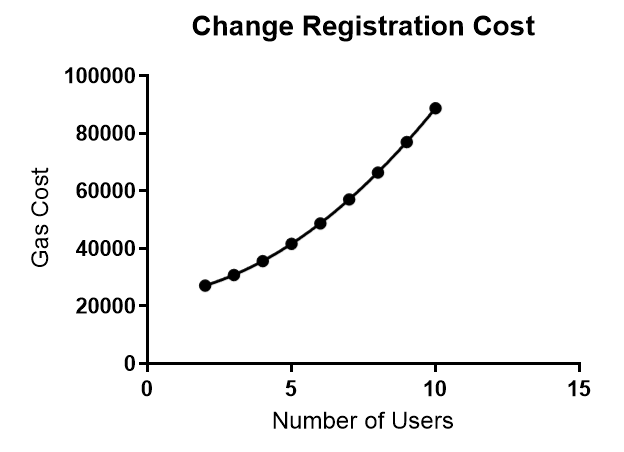
\includegraphics{cost}
\end{figure}
I preformed a quadratic regression. This gave me the formula $23235 + 809.9x + 573.6x^2$  with x being the number of users.. From this I could see that although the algorithm scales exponentially, the exponential coefficient are relatively low, and the majority of the gas cost comes from the constant coefficient unless there is a very large number of users. 
\subsection{End Vote}
This has two parameters; number of votes and number of candidates. I will assume that each vote gives a full ranking of candidates. This gave me this data.;
\begin{figure}[H]
\includegraphics{VotingAlgo}
\end{figure}
I then performed quadratic regression on each number of votes. This gave me these formulas with $x$ being the number of candidates.
\begin{gather*}
2 Votes Gas Cost = 34949 + 34583x + 1785x^2 \\
3 Votes Gas Cost = 41603 + 33925x + 2415x^2 \\
4 Votes Gas Cost = 45277 + 34952x + 3329x^2 \\
5 Votes Gas Cost = 52040 + 34431x + 3868x^2 \\
6 Votes Gas Cost = 59087 + 33107x + 5122x^2 \\
7 Votes Gas Cost = 61946 + 34583x + 5139x^2 \\
\end{gather*}
From this we can see that both increasing number of votes and number of candidates increases gas cost. However, we can also see that when there are more candidates, increasing the number of votes, increases the gas cost by more. We can also see that increasing number of candidates has a much greater impact than increasing number of votes.\\
This should scale well, as there should be considerably more votes than candidates. However there is no limit on the number of candidates and so the number of candidates could be the number of registered users. One way this could be solved is by removing all candidates at the end who have received 0 votes. This should stop users who are applying to representatives, to increase the gas cost of the voting algorithm. A problem with this solution is that it will increase the base cost of the function.
\subsection{Decide Budget}
This has five parameters number of representatives; number of sinks, coalition size factor, coalition size factor increase, and quota. For all my scaling tests, I will set quota to a majority of the total weights and collation size factor increase to one. \\
The first scaling test was how number of representatives affected gas cost. I set number of sinks to two and coalition size factor to 20. This gave me this data;
\begin{figure}[H]
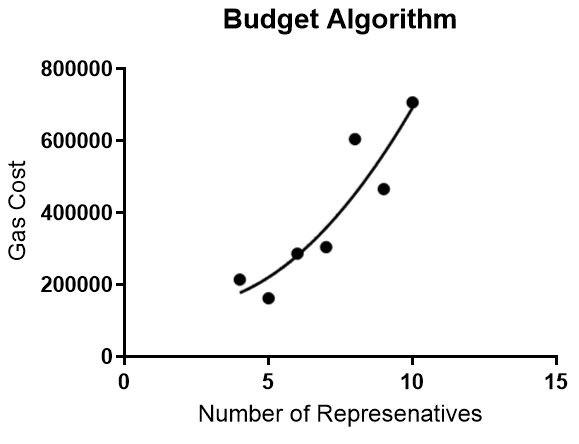
\includegraphics{budgetReps}
\end{figure}
I performed quadratic regression on the data again giving me this formula.  With $x$ being the number of representatives.
$Gas Cost = 175449 – 33592x + 8521x^2$ \\
From this I could see that my budget algorithm would not scale well, even with a moderate number of representatives. For example, 15 representatives would cost 1528044.
Another pattern I noticed was that if $n$ is number of representatives and $n$ is odd, then it costs less gas that $n – 1$. This can be explained, by my scaling test, setting the quota to be the majority of representatives, and so $n$ and $n – 1$ would need the same quota, but $n$ had more options to form coalitions with. \\
The next test was to see how the number of sinks affected the gas cost. I also created two series; one with 5 representatives and one with 7, to test if that affected the impact of increasing sinks. The data was as follows; \\
\begin{figure}[H]
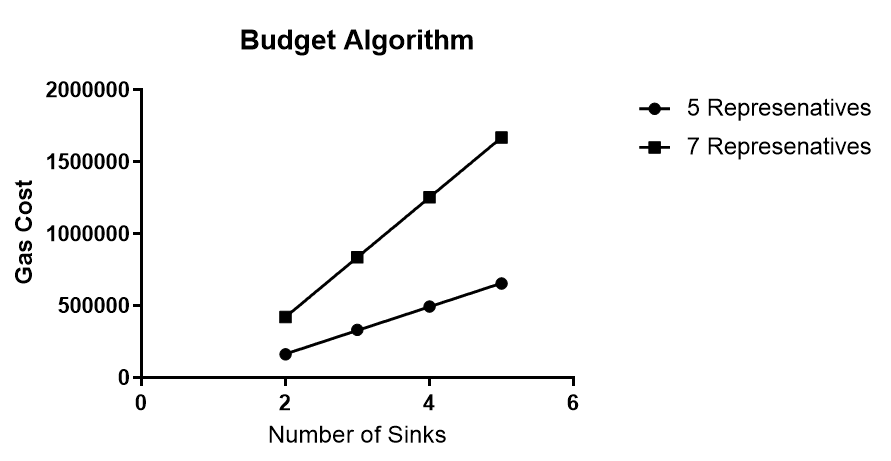
\includegraphics{budgetSinks}
\end{figure}
I then performed linear regression, giving me these formulas.  With $x$ being the number of sinks;
\begin{gather*}
5 Representatives Gas Cost = -162873 + 163827x \\
7 Representatives Gas Cost = -162873 + 163827x
\end{gather*}
From this I could see that increasing the number of sinks linearly increased the gas cost. However, when there is more representatives, the slope is much steeper. \\
The last test was how coalition size factor affected the gas cost. Again, I created two series; one with 5 representatives and one with 7. This gave me this data;\\
\begin{figure}[H]
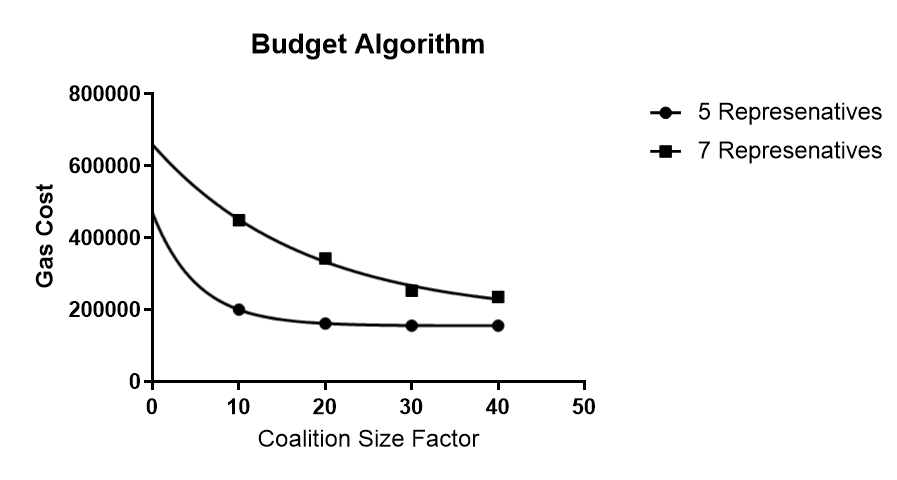
\includegraphics{budgetCoalitionSizeFactor}
\end{figure}
Then I performed a exponential decay regression. This created these functions. With $x$ being the number of representatives;
\begin{gather*}
5 Representatives Gas Cost = (469581 - 155443)*e^{(-0.19x)} + 155443 \\
7 Representatives Gas Cost = (658793 - 180286)*e^{(-0.05705x)} + 180286
\end{gather*}
From this I can see that that increasing coalition size factor decreases the gas cost. The plateau is reached when coalition size factor is so big, that agents always join the coalition with the biggest size. Therefore, coalitions can not be made any faster. \\
The coalition size factor should be chosen to keep the gas cost down to manageable level but care must be taken to not make it too large, that that larger coalitions are able to take all the utility in the negotiations. For example with 5 representatives, with a 30 starting coalition size factor, each agent just joins the largest coalition. \\
Another point to notice, is that budget negotiations with less representatives reach a plateau from increasing coalition size factor much quicker.  From this we can see that the more representatives, the larger we should start the coalition size factor, but with a small number we risk making negotiations too one sided.\\
\section{Fairness} 
\subsection{Voting Algorithm}
To measure my voting algorithm fairness, I created a google forms questionnaire. It asked users to rank crisp flavours from 1 to 5. It then used all the previous answered questions and the current users ranking with my voting algorithm and showed the user the current result of the voting algorithm. It then asked the user to rate the result Very Fair / Fair / Don’t Know / Unfair / Very Unfair. To allow me to return a result to the first user, I also created 5 dummy votes. \\
The reason I choose to collect crisp flavour votes is that it is non-sensitive data, that users would be able to quickly be able to answer, and also because it’s a subject the users know about, and the user will care about the result and therefore be able to put how happy he is with the result. \\
I then sent the google forms link to the computer science group chat. 12 users answered my survey. The modal result was Fair and the median result was 4.2 (Very Unfair being 1 and Very Fair being 5). I will evaluate my voting algorithm as being fair enough, however 12 users is a small sample size and so more research will need to be done.
\subsection{Budget Algorithm}
To measure my budget algorithm fairness, I also created a google forms questionnaire. This showed users all the budgets of the representatives and showed the result of my algorithm. It then asked users to rate the result with the same Likert scale I used with my voting algorithm.  \\
Again, I then sent the google forms link to the computer science group chat. 9 users answered my survey. The modal result was Fair and the median result was 3.8. Although most users choose fair, a few users thought the result was unfair. I need to do more research to change my algorithm, ensuring more users believe the result to be fair and to find out what is currently wrong with my algorithm.
